% This work is licensed under the Creative Commons Attribution-NonCommercial-NoDerivs
% 3.0 Unported License. To view a copy of this license, visit
% http://creativecommons.org/licenses/by-nc-nd/3.0/ or send a letter to
% Creative Commons, 444 Castro Street, Suite 900, Mountain View, California, 94041, USA.

%-------------------------------------------------------------------------------
\begin{frame}\frametitle{Cherry-pick}
  "Cueille" un commit et l'applique sur la branche courante.\\
  \alert{git cherry-pick 1b308c6}
\end{frame}
%-------------------------------------------------------------------------------
\begin{frame}\frametitle{Reflog}
  Journal des activités sur le repo local\\
  $-->$ le sauveur après un git reset --hard HEAD~2 trop rapide.

\end{frame}
%-------------------------------------------------------------------------------
\begin{frame}\frametitle{Amend}
Ne crée pas de nouveau commit, se contente d'éditer le dernier.\\
  \alert{git commit --amend}\\
  bonus : --no-edit

\end{frame}
%-------------------------------------------------------------------------------
\begin{frame}[fragile]\frametitle{Show}
  Afficher le contenu d'un fichier sur une autre branche :\\
  \alert{git show other\_branch:some\_file.txt}

\end{frame}
%-------------------------------------------------------------------------------
\begin{frame}\frametitle{Rebase : réécriture d'historique}
  \begin{center}
    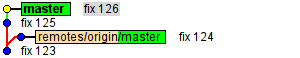
\includegraphics[width=0.7\textwidth]{./images/rebase-0.png}
  \end{center}
  \alert{git pull --rebase}
  \begin{center}
    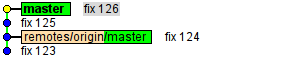
\includegraphics[width=0.7\textwidth]{./images/rebase-1.png}
  \end{center}

\end{frame}
%-------------------------------------------------------------------------------
\begin{frame}\frametitle{Rebase : danger}
Réécrire l'historique peut être lourd de conséquences !
\begin{itemize}
  \item risque de perte de commit
  \item risque d'avoir plusieurs versions d'un même commit
\end{itemize}

\end{frame}
%-------------------------------------------------------------------------------
\begin{frame}[fragile]\frametitle{Stash}
  Mettre des changements de coté: \alert{git stash}\\
\textit{to stash}: planquer, mettre dans une cachette
\end{frame}
%-------------------------------------------------------------------------------
\begin{frame}\frametitle{Dépôt central}
  \begin{center}
    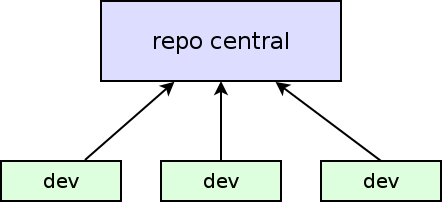
\includegraphics[width=0.7\textwidth]{./images/repo_central.png}
  \end{center}
  \begin{itemize}
    \item mise en place rapide
    \item pas de mécanisme de protection du dépôt central
  \end{itemize}

\end{frame}
%-------------------------------------------------------------------------------
\begin{frame}\frametitle{Integration manager}
  \begin{center}
    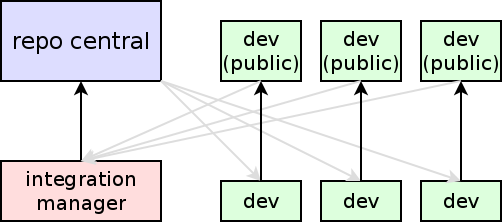
\includegraphics[width=0.7\textwidth]{./images/integration_manager.png}
  \end{center}
  \begin{itemize}
    \item plus de contrôle sur le branches du dépôt central
    \item peu adapté à des équipes importantes
  \end{itemize}

\end{frame}
%-------------------------------------------------------------------------------
\begin{frame}\frametitle{Dictateur - lieutenants}
  \begin{center}
    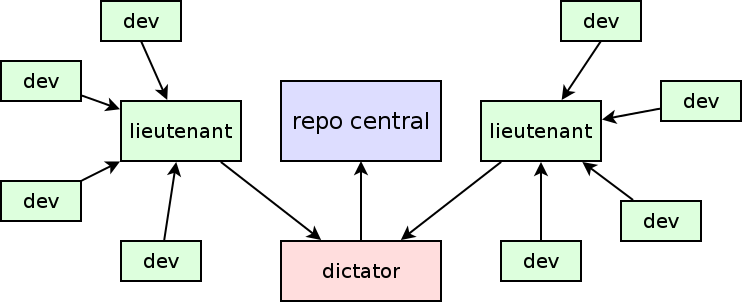
\includegraphics[width=0.8\textwidth]{./images/dictator.png}
  \end{center}
  \begin{itemize}
    \item permet de répartir les responsabilités
    \item adapté à des équipes (très) importantes
  \end{itemize}
\end{frame}

%-------------------------------------------------------------------------------
\begin{frame}\frametitle{TP : bac à sable avancé}
  rebase, reflog, stash
\end{frame}

% max 80 columns : merges become messy with pure text and longer lines.
% vim: set colorcolumn=+1 textwidth=80:
